\documentclass[11pt,a4paper]{article}
\usepackage[margin=2.2cm]{geometry}
\usepackage{amsmath}
\usepackage{graphicx}
\usepackage{float}
\usepackage{listings}

\lstset{basicstyle=\ttfamily\footnotesize, frame=single, numbers=left,
        numberstyle=\tiny, breaklines=true, columns=fullflexible, showstringspaces=false}

\title{DEP521E -- HW3 Part C\\Newton-Raphson Iteration with Newmark-$\beta$ (Coded with AI)}
\author{Mesut ADALI - 801262107}
\date{16.11.2026}

\begin{document}
\maketitle

\section{Scope}
The code of Section 1 (original Newton-Raphson iteration with the Newmark-$\beta$ solver)
was developed with an AI tool (Claude, Anthropic). The same bilinear spring model of HW2
is used. The script also has a \texttt{--modified} option for the modified Newton-Raphson
algorithm, which keeps the stiffness of the start of the step during the iterations.

\section{Input Parameters}
\begin{table}[H]
\centering
\begin{tabular}{llrl}
\hline
Parameter & Symbol & Value & Units \\
\hline
Mass                & $m$   & 1000    & kg \\
Damping ratio       & $\xi$ & 2       & \% \\
Initial period      & $T$   & 1       & s \\
Primary stiffness   & $k_p = m(2\pi/T)^2$ & 39478.4 & N/m \\
Yield displacement  & $d_y$ & 7.5     & cm \\
Yield force         & $f_y = k_p d_y$ & 2960.9 & N \\
Secondary stiffness & $k_s = 0.1k_p$  & 3947.8 & N/m \\
Damping coefficient & $c = 2\xi m\omega_n$ & 251.33 & N\,s/m \\
\hline
\end{tabular}
\caption{SDOF system parameters.}
\end{table}
The ground acceleration of HW1 is used ($\Delta t = 0.005$~s, 7860 points). The values
are in g, so they are multiplied by 9.806 to get m/s$^2$. The load is $p = -m\ddot{u}_g$.

\section{Method}
The average acceleration method is used ($\beta = 1/4$, $\gamma = 1/2$). Because the
spring force $f_s(u)$ is nonlinear, the total form of Newmark-$\beta$ is solved at each step:
\[
\hat{p}_{i+1} = p_{i+1} + a_1 u_i + a_2 \dot{u}_i + a_3 \ddot{u}_i
\]
\[
a_1 = \frac{m}{\beta\Delta t^2} + \frac{\gamma c}{\beta\Delta t}, \qquad
a_2 = \frac{m}{\beta\Delta t} + \left(\frac{\gamma}{\beta}-1\right)c, \qquad
a_3 = \left(\frac{1}{2\beta}-1\right)m + \Delta t\left(\frac{\gamma}{2\beta}-1\right)c
\]
The equation $f_s(u_{i+1}) + a_1 u_{i+1} = \hat{p}_{i+1}$ is solved with Newton-Raphson.
Starting from $u^{(0)} = u_i$, at each iteration $j$:
\[
R^{(j)} = \hat{p}_{i+1} - f_s^{(j)} - a_1 u^{(j)}, \qquad
\hat{k}_T^{(j)} = k_T^{(j)} + a_1, \qquad
u^{(j+1)} = u^{(j)} + R^{(j)}/\hat{k}_T^{(j)}
\]
\begin{itemize}
  \item $f_s^{(j)}$ is found with the bilinear function of HW2. The function is always called
        from the converged state of the start of the step ($u_i$, $f_{s,i}$, state$_i$) with
        $\Delta u = u^{(j)} - u_i$, so the trial iterations do not add false plastic deformation.
  \item Tangent stiffness: $k_T = k_p$ in the Interior Region and $k_T = k_s$ on the Top or Bottom Border.
  \item Original algorithm: $k_T$ is updated at every iteration.
        Modified algorithm: $k_T$ of the start of the step is used for all iterations.
  \item Convergence: $|f^{(j+1)}_{s,ub}| / |f^{(j)}_{s,ub}| < 0.01$, where $f_{s,ub} = R$ is the
        unbalanced force after an iteration. A zero unbalanced force (elastic step) is also accepted.
\end{itemize}
After convergence the velocity and acceleration are updated:
\[
\dot{u}_{i+1} = \frac{\gamma}{\beta\Delta t}(u_{i+1}-u_i) + \left(1-\frac{\gamma}{\beta}\right)\dot{u}_i
              + \Delta t\left(1-\frac{\gamma}{2\beta}\right)\ddot{u}_i
\]
\[
\ddot{u}_{i+1} = \frac{u_{i+1}-u_i}{\beta\Delta t^2} - \frac{\dot{u}_i}{\beta\Delta t}
               - \left(\frac{1}{2\beta}-1\right)\ddot{u}_i
\]
The absolute acceleration is $\ddot{u}_{abs} = \ddot{u} + \ddot{u}_g$.

\section{Command Line Output}
\begin{lstlisting}
Original Newton-Raphson + Newmark-beta (beta = 1/4, gamma = 1/2), dt = 0.005 s
kp = 39478.4 N/m, fy = 2960.9 N, ks = 3947.8 N/m, c = 251.33 N s/m
Steps: 7859, steps on a yield border: 194
Iterations in yielding steps: 1 iter -> 189 steps, 2 iter -> 5 steps
  max = 2, mean = 1.03
Total iterations: 7869
Max |x| = 21.461 cm, max |fs| = 3512.0 N, max |v| = 0.8409 m/s, max |a_abs| = 3.5446 m/s^2
Analysis time: 0.0187 s
\end{lstlisting}

\section{Results}
\begin{figure}[H]
\centering
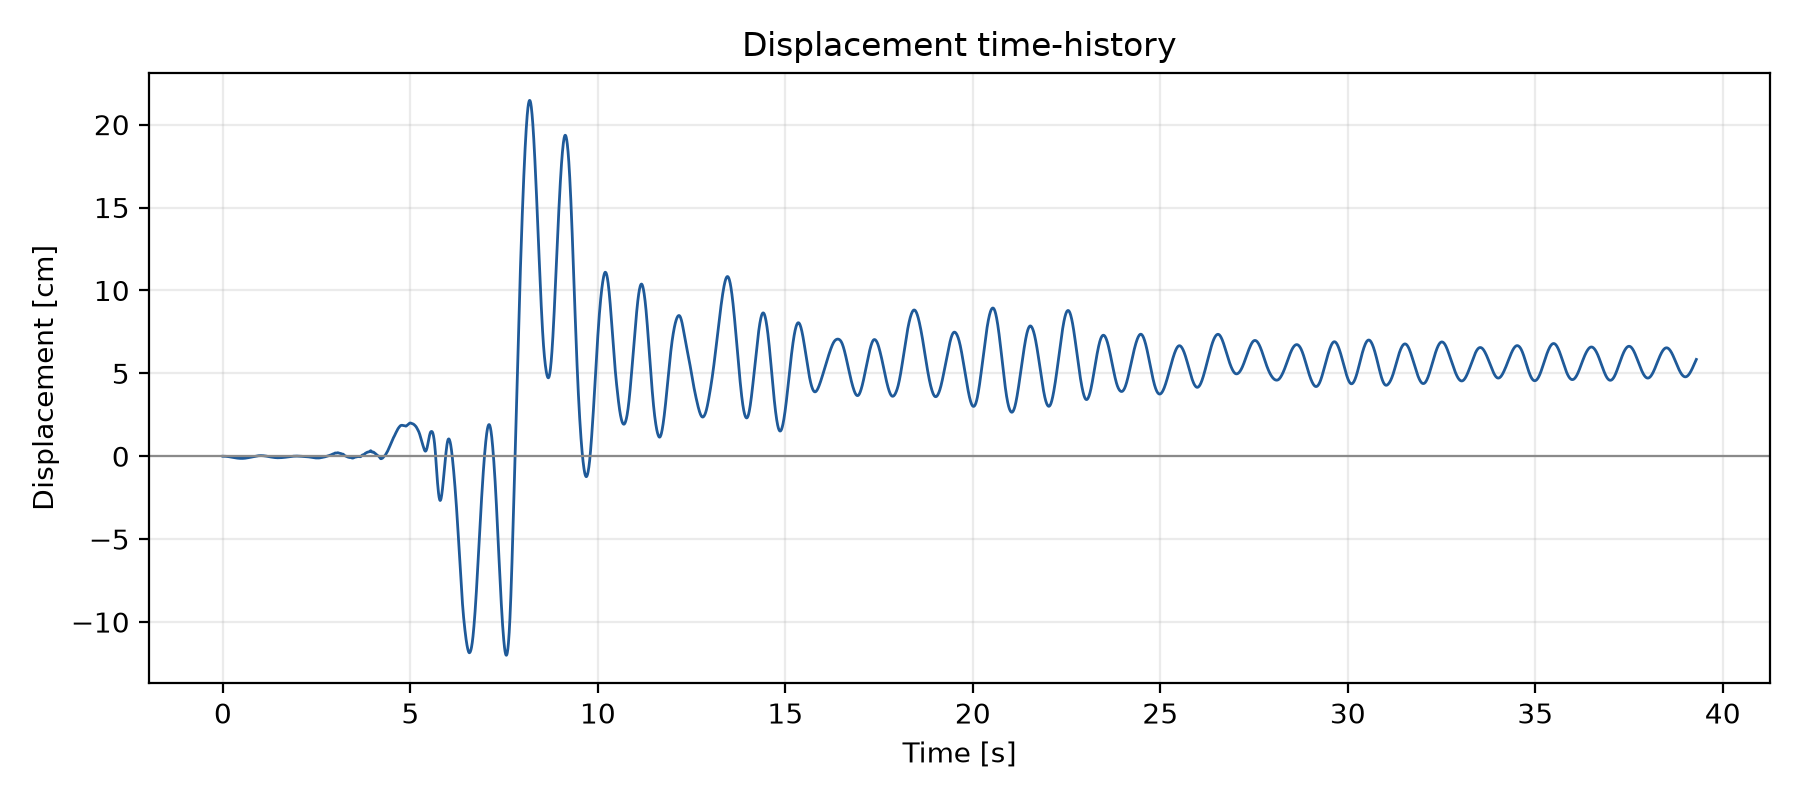
\includegraphics[width=0.49\textwidth]{figures/displacement_history.png}
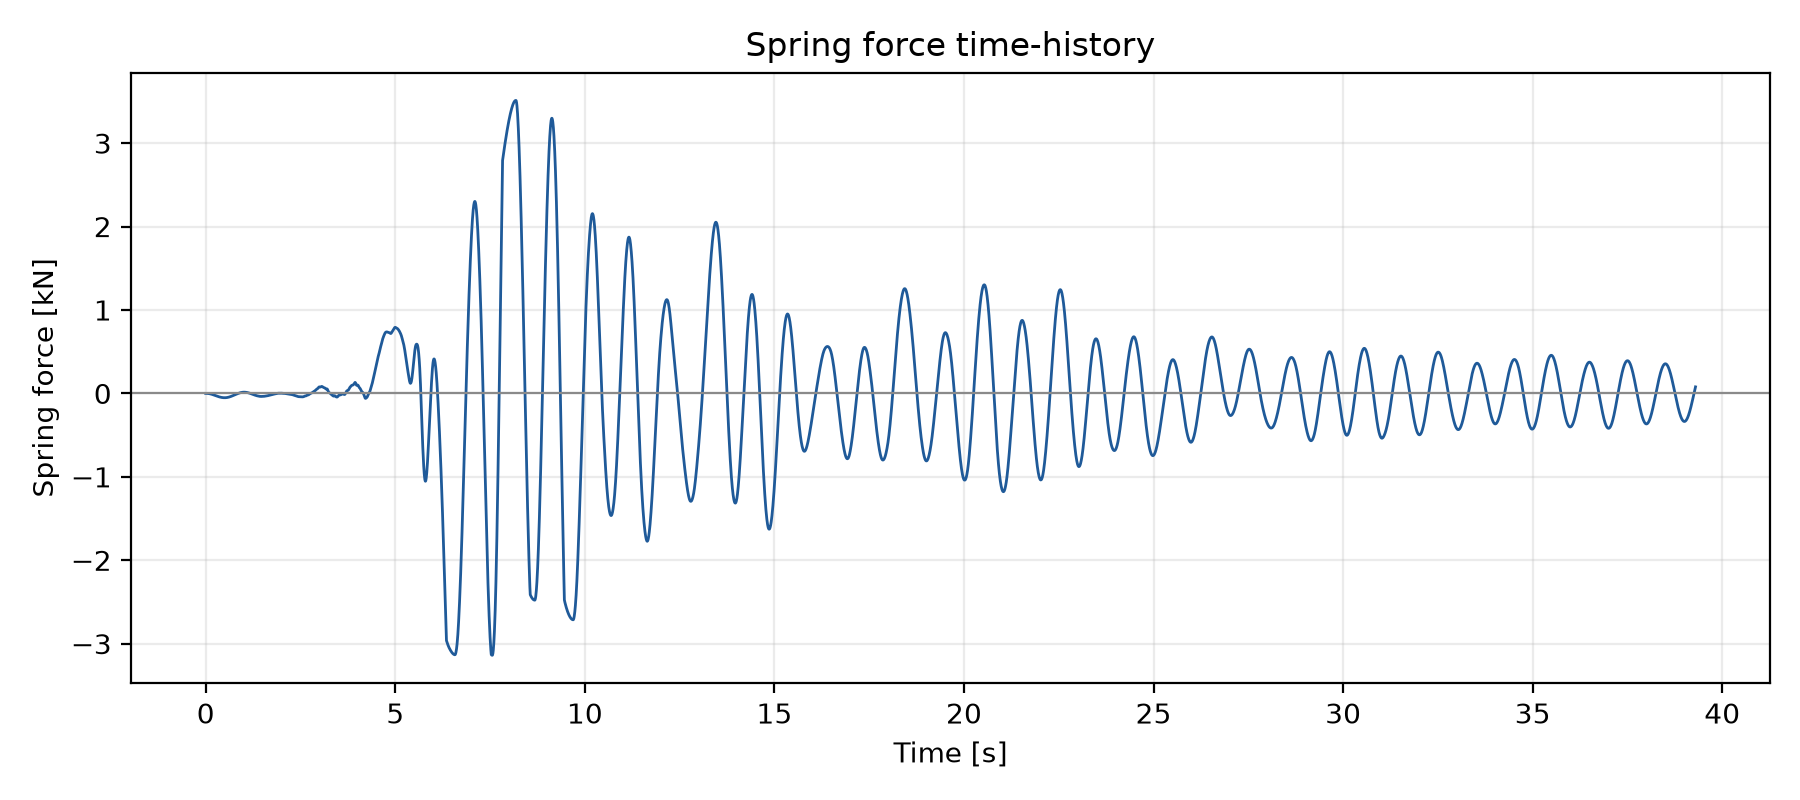
\includegraphics[width=0.49\textwidth]{figures/spring_force_history.png}
\caption{Displacement time history (left) and spring force time history (right).}
\end{figure}

\begin{figure}[H]
\centering
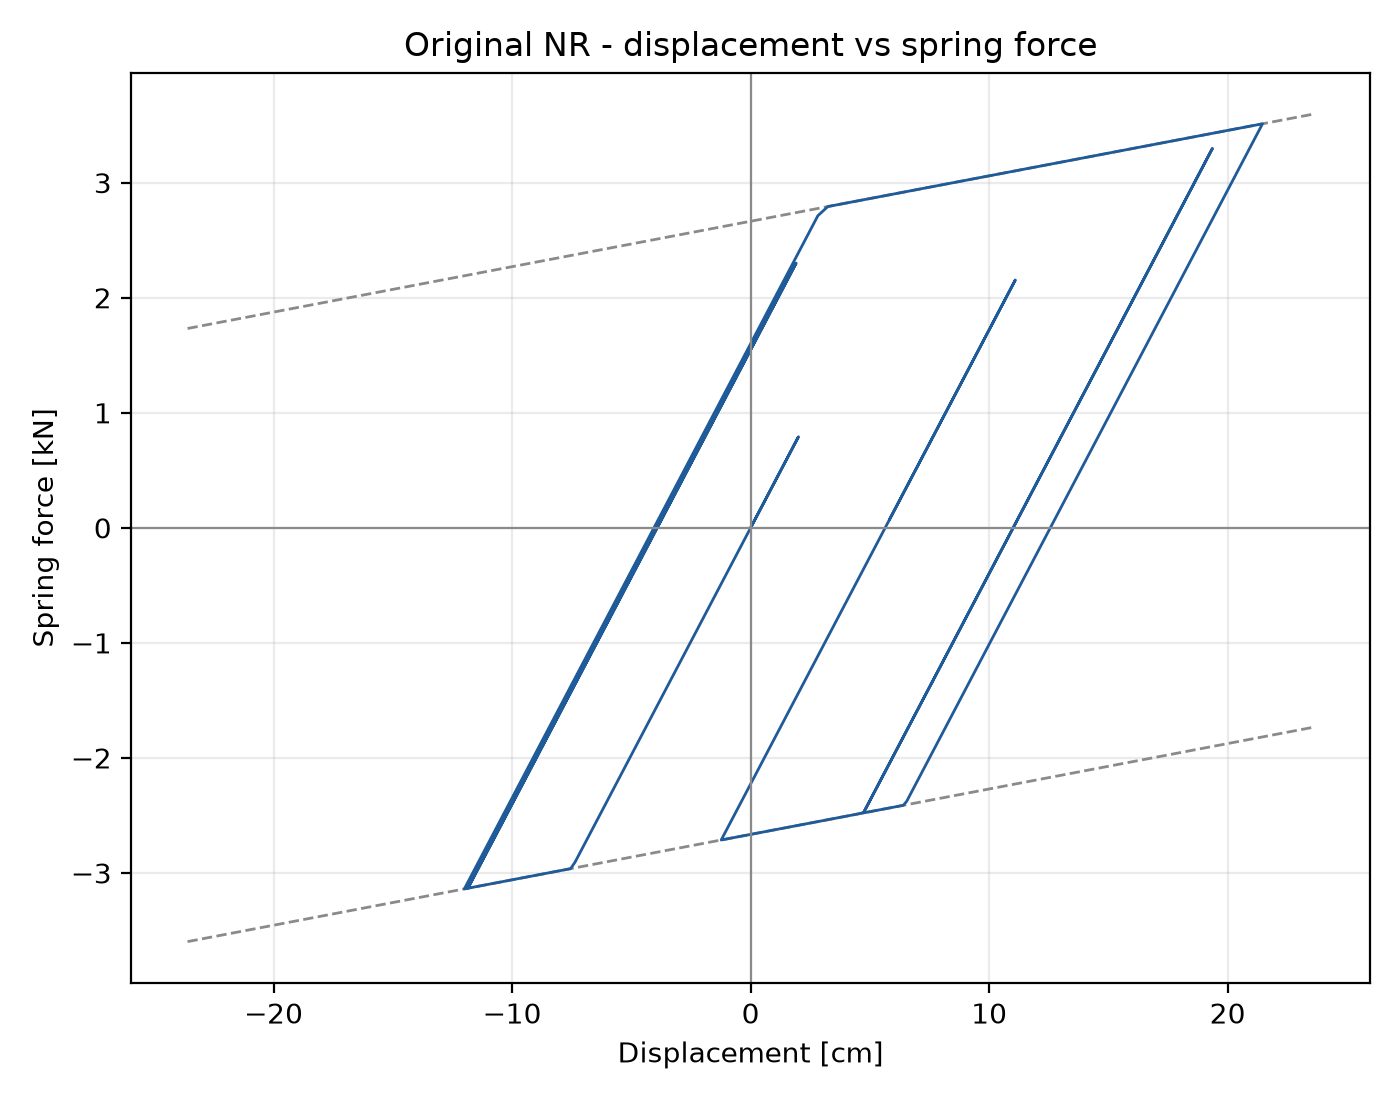
\includegraphics[width=0.6\textwidth]{figures/hysteresis.png}
\caption{Displacement -- spring force hysteresis. Dashed lines are the Top and Bottom Borders.}
\end{figure}

\begin{figure}[H]
\centering
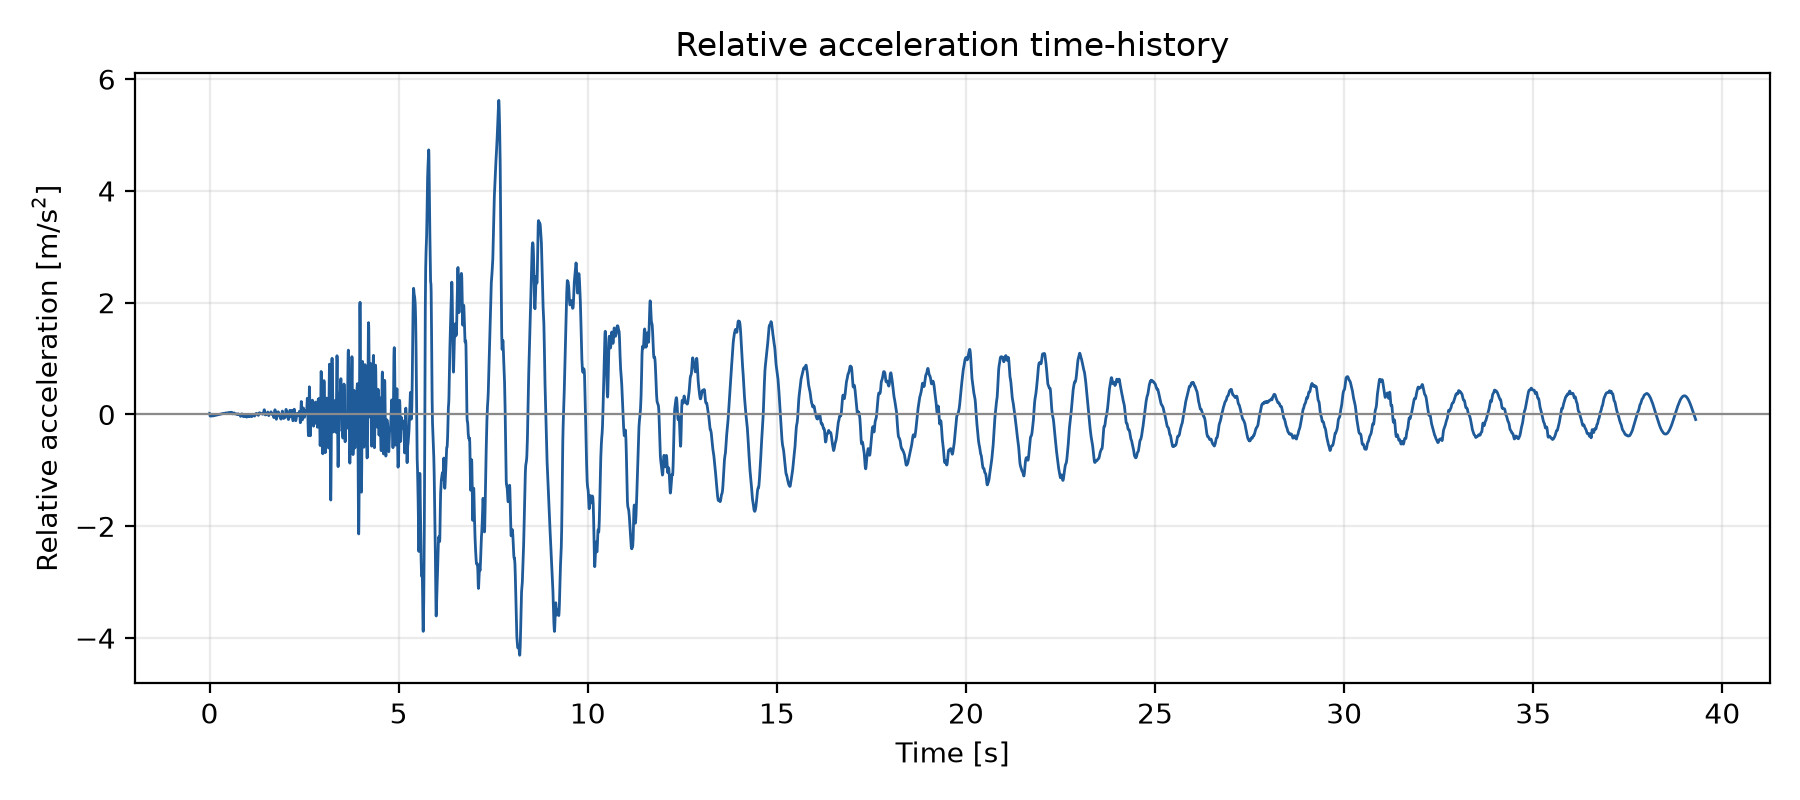
\includegraphics[width=0.49\textwidth]{figures/relative_acceleration_history.png}
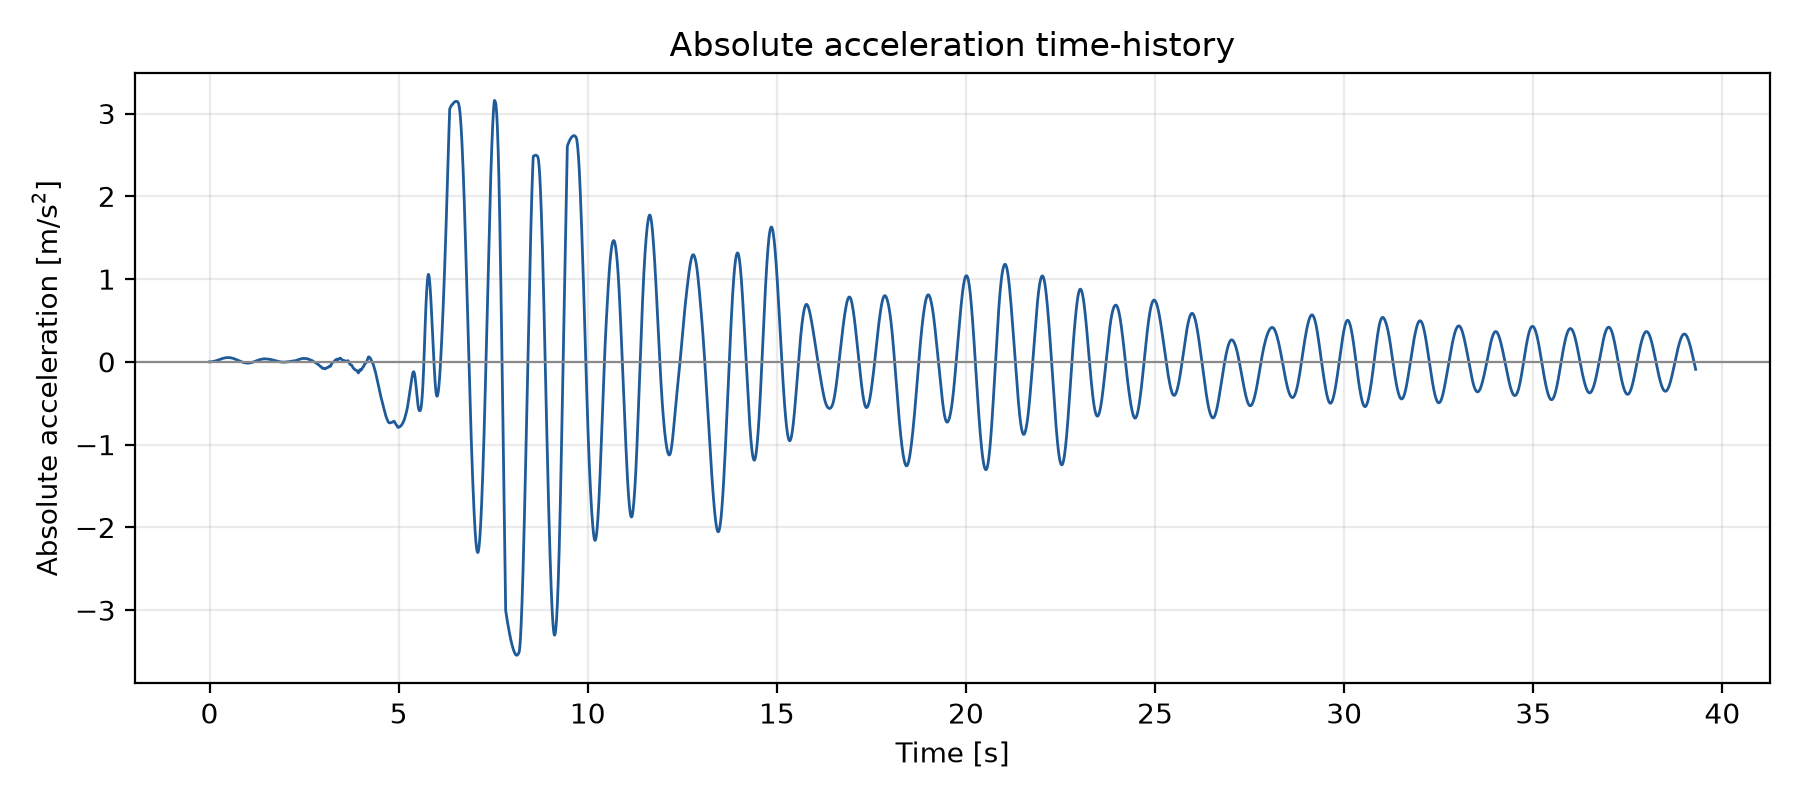
\includegraphics[width=0.49\textwidth]{figures/absolute_acceleration_history.png}
\caption{Relative acceleration (left) and absolute acceleration (right) time histories.}
\end{figure}

\section{Discussion}
\begin{itemize}
  \item The system first yields at $t = 6.35$~s. The maximum displacement is 21.46~cm and the
        maximum spring force is 3512~N. After the motion a residual displacement of about 5.7~cm remains.
  \item 194 of 7859 steps end on a yield border. 189 of them converge in 1 iteration and 5 of them
        in 2 iterations. The steps with 2 iterations are the steps where the spring passes from the
        Interior Region to a border: the first trial uses $k_p$, the second uses $k_s$ and is exact,
        because the bilinear model is linear on each branch.
  \item The modified algorithm gives the same iteration counts and the same results. The reason is the
        small time step: $a_1 = m/(\beta\Delta t^2) \approx 1.6\times10^8$~N/m is about 4000 times $k_p$,
        so updating the spring stiffness changes $\hat{k}_T$ very little.
  \item Check: the equilibrium $m\ddot{u} + c\dot{u} + f_s = p$ is satisfied at every step with an error
        below $10^{-8}$~N. With a very large $d_y$ (no yielding) the result is equal to the linear
        Newmark-$\beta$ solution of HW1 within $10^{-13}$~m.
\end{itemize}

\appendix
\section{Python Code}
\lstinputlisting[language=Python]{nr_newmark.py}

\end{document}
